
%(BEGIN_QUESTION)
% Copyright 2012, Tony R. Kuphaldt, released under the Creative Commons Attribution License (v 1.0)
% This means you may do almost anything with this work of mine, so long as you give me proper credit

The following circuit controls the starting and stopping of a motor-driven air compressor.  The ``M'' coil is the coil of a three-phase contactor relay sending 480 VAC to the compressor's electric motor.  The ``OL'' contact is a thermal overload contact (similar to a ``51'' time-overcurrent protective relay) which forces the contactor to de-energize and cut power to the motor if the motor draws too much current over time:

$$\includegraphics[width=15.5cm]{i02110x01.eps}$$

Suppose you were asked to test the high-pressure ``cut-out'' switch for proper operation without shutting the compressor down to perform the test.  Explain how you could perform this test safely while the compressor was running.

\vskip 10pt

Also, calculate the PFD for unchecked overpressure (substantially above 110 PSI) given the following pressure switch dependability values, assuming the hand switch is left in the ``Auto'' position:

\begin{itemize}
\item{} Dependability$_{control}$ = 0.947 
\item{} Dependability$_{cutout}$ = 0.981
\end{itemize}

\vskip 20pt \vbox{\hrule \hbox{\strut \vrule{} {\bf Suggestions for Socratic discussion} \vrule} \hrule}

\begin{itemize}
\item{} Identify any safety precautions to follow when working on a ``live'' 120 VAC circuit (e.g. the {\it one-hand} rule).
\item{} How would the PFD of this system be affected if the hand switch were left in the ``Hand'' position?
\end{itemize}

\underbar{file i02110}
%(END_QUESTION)





%(BEGIN_ANSWER)

$\hbox{PFD} = 0.001007$

%(END_ANSWER)





%(BEGIN_NOTES)

In order to test the high-pressure cutout switch, we could first jumper its terminals electrically so that the circuit will remain powered when the switch contacts open.  Next, we can shut the block valve for that PSH and disconnect it from the circuit (as well as remove it from the vessel) and bring the switch back to the shop for testing.

\vskip 10pt

Since this is a 1oo2 trip system, the probability that the system will reliably trip when needed is an OR function of the two switches' dependabilities (in other words, either one switch or the other needs to be dependable in order to avoid an overpressure condition):

$$P(\hbox{A {\it or} B}) = P(B) + P(A) - P(A) \times P(B)$$

$$\hbox{Dependability}_{1oo2} = 0.947 + 0.981 - (0.947)(0.981)$$

$$\hbox{Dependability}_{1oo2} = 0.998993$$

Since we are looking for the probability that both these switches will fail to stop an overpressure condition, the PFD will be the complement of this 1oo2 reliability:

$$PFD = 1 - \hbox{Dependability}$$

$$\hbox{PFD}_{1oo2} = 0.001007$$

$$\includegraphics[width=15.5cm]{i02110x02.eps}$$

%INDEX% Electronics review: AC motor control circuit
%INDEX% Process: air compressor and receiver tank
%INDEX% Safety, shutdown system: trip testing 
%INDEX% Safety, system reliability: probability of failure on demand (PFD)

%(END_NOTES)


